\newpage

\chapter*{Abstract}


\begin{slshape}
%change to master thesis
%In this literature study we will attempt to clearly state the research question and provide adequate background. This should provide us with enough information to start working on the actual research problem. We will provide a roadmap trying to answer this question and the clearly map the path that will be followed and where potential issues might arise. We will also elaborate on why this research question is relevant at this current time. 

%\npar

%The literature study is constructed as follows. First we will describe the origin of the internet and look at how the internet got to where it is right now. In the same chapter we will inspect some other alternatives proposed for internet throughout the years. We will conclude the chapter with some of the shortcomings the current internet model faces. In the following chapter we will state the main research question alongside with the specifics this question poses. Following the main question we will explain the basics of Recursive InterNetworking Architecture (RINA), take a closer look at the IRATI implementation of RINA and finish with the restrictions we might encounter for the Android platform. The next chapter will be specifically about RINA on the android platform with specific sections about the wireless Shim-DIF and WiFi Media Access Control. The final chapter intends to draw a conclusion about the literature study and show the position of the study in the whole thesis.

%\npar

%%This Master's Thesis aims to provide insight in the Recursive InterNetwork Architecture over wireless on Android. With the current Internet evolving at an accelerating rate, we note that the jungle of protocols is becoming more difficult to understand with each step of this evolution. A closer look at the current architecture reveals many flaws and notices that several updates are simply patches to make the current Internet workable. A simple example is the old IP protocol which is now running out of addresses (IPv6), so we have to patch it with a similar protocol which adds very little functionality (IPv6). The Recursive InterNetwork Architecture (RINA) is an alternative to the current Internet. This Master Thesis will provide understanding of this new architecture. At the same time do we intend to implement RINA over wireless medium (WiFi protocol) on Android operating system.

%%\npar

%%The Master's Thesis is constructed in the following manner. First we will provide an introduction chapter which focuses on providing an adequate initiation about the architecture. Following this we present the literature study. This literature study initiates with the origin of the Internet and looks at how the Internet got to where it is now. In the same section we will inspect some other alternatives proposed for internet throughout the years. We will conclude the section with some of the shortcomings the current internet model faces. In the following section we will state the main research question alongside with the specifics this question poses. Following the main question we will explain the basics of Recursive InterNetwork Architecture (RINA), take a closer look at the IRATI implementation of RINA and finish with the restrictions we might encounter for the Android platform. The next section will be specifically about RINA on the android platform with specific subsections about the Wireless Shim DIF and WiFi Media Access Control. The final section intends to draw a conclusion about the literature study and show the position of the study in the whole thesis.

%%\npar

%%Following the literature study chapter we dedicate a chapter to the Specification of the Shim DIF over WiFi. This specification provides enough information to build a Shim DIF over WiFi. This specification is specifically tailored to the IRATI project. It also supplies the reader with enough information to understand the lowest level DIF. In addition to that the reader also gains valuable insight in the entire Recursive InterNetwork Architecture (RINA). 

%%\npar

%%After the Specification we dedicate a chapter to the implementation of RINA on Android over WiFi. After the literature study we have actually come to the conclusion that WiFi is unreachable by the architecture in its current form. This means that this implementation will greatly focus on adapting the current codebase to the Android operating system. The chapter consists of a first section which states the plan of action of the implementation. After a quick introduction and the procedure of implementation we move to the next section, proof of concept over WiFi. Here we implement the current IRATI stack, explain the basics of kernel compilation and implement the IRATI code. This implementation is done on two physical Linux machines which communicate with each other over WiFi. Finally the last section of this chapter moves towards the implementation of RINA on Android. The section is further divided to list the different requirements that need to be met before an actual implementation on Android can be acquired. 

%%\npar

%%The final chapter provides a conclusion for the Master's Thesis. It will clearly show the plan of action that was taken to get to the answer on the research question. Finally, the research question will be fully answered. This will conclude the Master's Thesis and in total this should provide an adequate amount of information about the research question and similar topics. 


The current version of the Internet is a jungle of protocols. Generic protocols interfere with each other, modern protocols overlap with their outdated versions, old issues such as multihoming, layer boundaries, \ldots were never solved. It is clear we need a new architecture. 
\npar
With the Internet being born out of ARPANET, instantly several issues became noticeable. ARPANET was a proof of concept, it was never a research net. This means it was never suitable to be the foundation of the current Internet. Several research networks were constructed but were discontinued when ARPANET was moving towards a public network. Several protocols were added to ARPANET and finally it stepped out of its infancy and moved towards a public net. None of the issues were solved though. Protocols were added on top of this, issues that rose during the early stage were never addressed, but the expansion continued anyway. Recursive InterNetworking Architecture, RINA is an alternative architecture that offers an entire new architecture instead of one more protocol meant to patch one specific problem. RINA starts from the basic rule: ´´Networking is Inter Process Communication (IPC) and IPC only''. Every IPC has IPC processes that wish to communicate with each other. These IPC processes are bundled in a Distributed IPC Facility (DIF). These DIFs are stacked recursively on top of each other. Every DIF has the same mechanism, but different scopes and policies make these DIFs different. 

\npar

RINA is a theoretical architecture, without a technical implementation its use cannot be proven. The technical implementation we will be cooperating with is: ``Investigating RINA as Alternative to TCP/IP'', IRATI. This project aims to provide an implementation of RINA at the lowest possible layer that is currently feasible. While the lowest layer is simply the physical layer, for testing purposes this would prove to be fairly useless as this layer is not directly available in operating systems. This means placemet of the project's code has to be right on top of the link layer. The current existing prototype already provides a working Shim DIF for Ethernet. 
\begin{wrapfigure}{r}{0.28\textwidth}
	\centering
	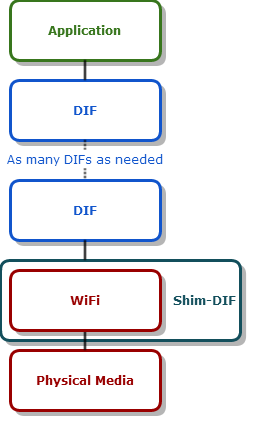
\includegraphics[width=0.25\textwidth]{figures/rinaoverwifi}
\end{wrapfigure}
A Shim DIF is a DIF which uses the functionality from the lower layer (e.g. Ethernet) and presents this as a DIF to the upper RINA DIF. Note that these Shim DIFs are not fully functional DIFs, but are needed to implement the code as low as possible. The goal is to construct a Shim DIF over WiFi on Android, based on the Shim DIF over Ethernet on Debian Wheezy. 
\npar
In Linux kernels and Linux-like kernels WiFi frames are being reconstructed as Ethernet frames. After this reconstruction these frames are presented to the kernel. This means that WiFi frames are inaccessible for the user, even the admin (root). In the future this could change or people who currently write the code for the devices which handle this reconstruction could be willing to add implementation for RINA. For this reason a specification will be written which stipulates how the Shim-DIF over WiFi should be constructed. This implementation is specific for the IRATI project.
\npar
The implementation on Android is composed through different approaches and a plethora of iterations. After the construction of the base kernel the attempt to add the IRATI specific code to the kernel is made. This proved to be impossible without drastic changes to the code. Other issues arise here as well, such as the addition of system calls to this Android kernel. Further obstacles, such a userspace implementation, package installation, C library incompatibility, \ldots all added to the difficulty of implementation. With the current timeframe, manpower, and knowledge the success of implementation on Android fell outside the scope of this Master's Thesis. 




\end{slshape}
